\section[AMBIENTE DE ESTUDO]{AMBIENTE DE ESTUDO}

Como este trabalho trata de um projeto de desenvolvimento de software na área de análise de marcha, dois ambientes de trabalho distintos foram amplamente utilizados. São estes:

\begin{enumerate}
	\item Laboratório de Informática em Saúde (LIS) na Faculdade Gama (FGA) da Universidade de Brasília (UnB);
	\item Laboratório de Performance Humana (LPH) na Faculdade Ceilândia (FCE) da UnB.
\end{enumerate}

No LIS foram desempenhadas as tarefas relativas a engenharia de software e disponibilização do software.
Foram utilizadas estações de trabalho do tipo \emph{Power Mac} com sistema operacional \emph{MAC OS X} 10.10.3, sendo que uma foi preparada para funcionar como servidor de aplicação e roteador de rede. 
A estação preparada serve de hospedeira de duas máquinas virtuais (\emph{Virtual Machines} - VMs) rodando através do software \emph{Virtualbox} 4.3. 
Cada VM utiliza sistema operacional \emph{Debian Wheezy GNU/Linux}. 
Uma destas VMs foi configurada como roteador e \emph{firewall} e a outra como servidor de aplicações.  
Outra estação de trabalho \emph{Power Mac}, idêntica, e um \emph{notebook} rodando \emph{Ubuntu 14.04 GNU/Linux} foram utilizados como máquinas de desenvolvimento e simulação.
Um diagrama da rede criada no LIS é mostrado na Figura \ref{lis_rede}.

\begin{figure}[ht]
	\centering
	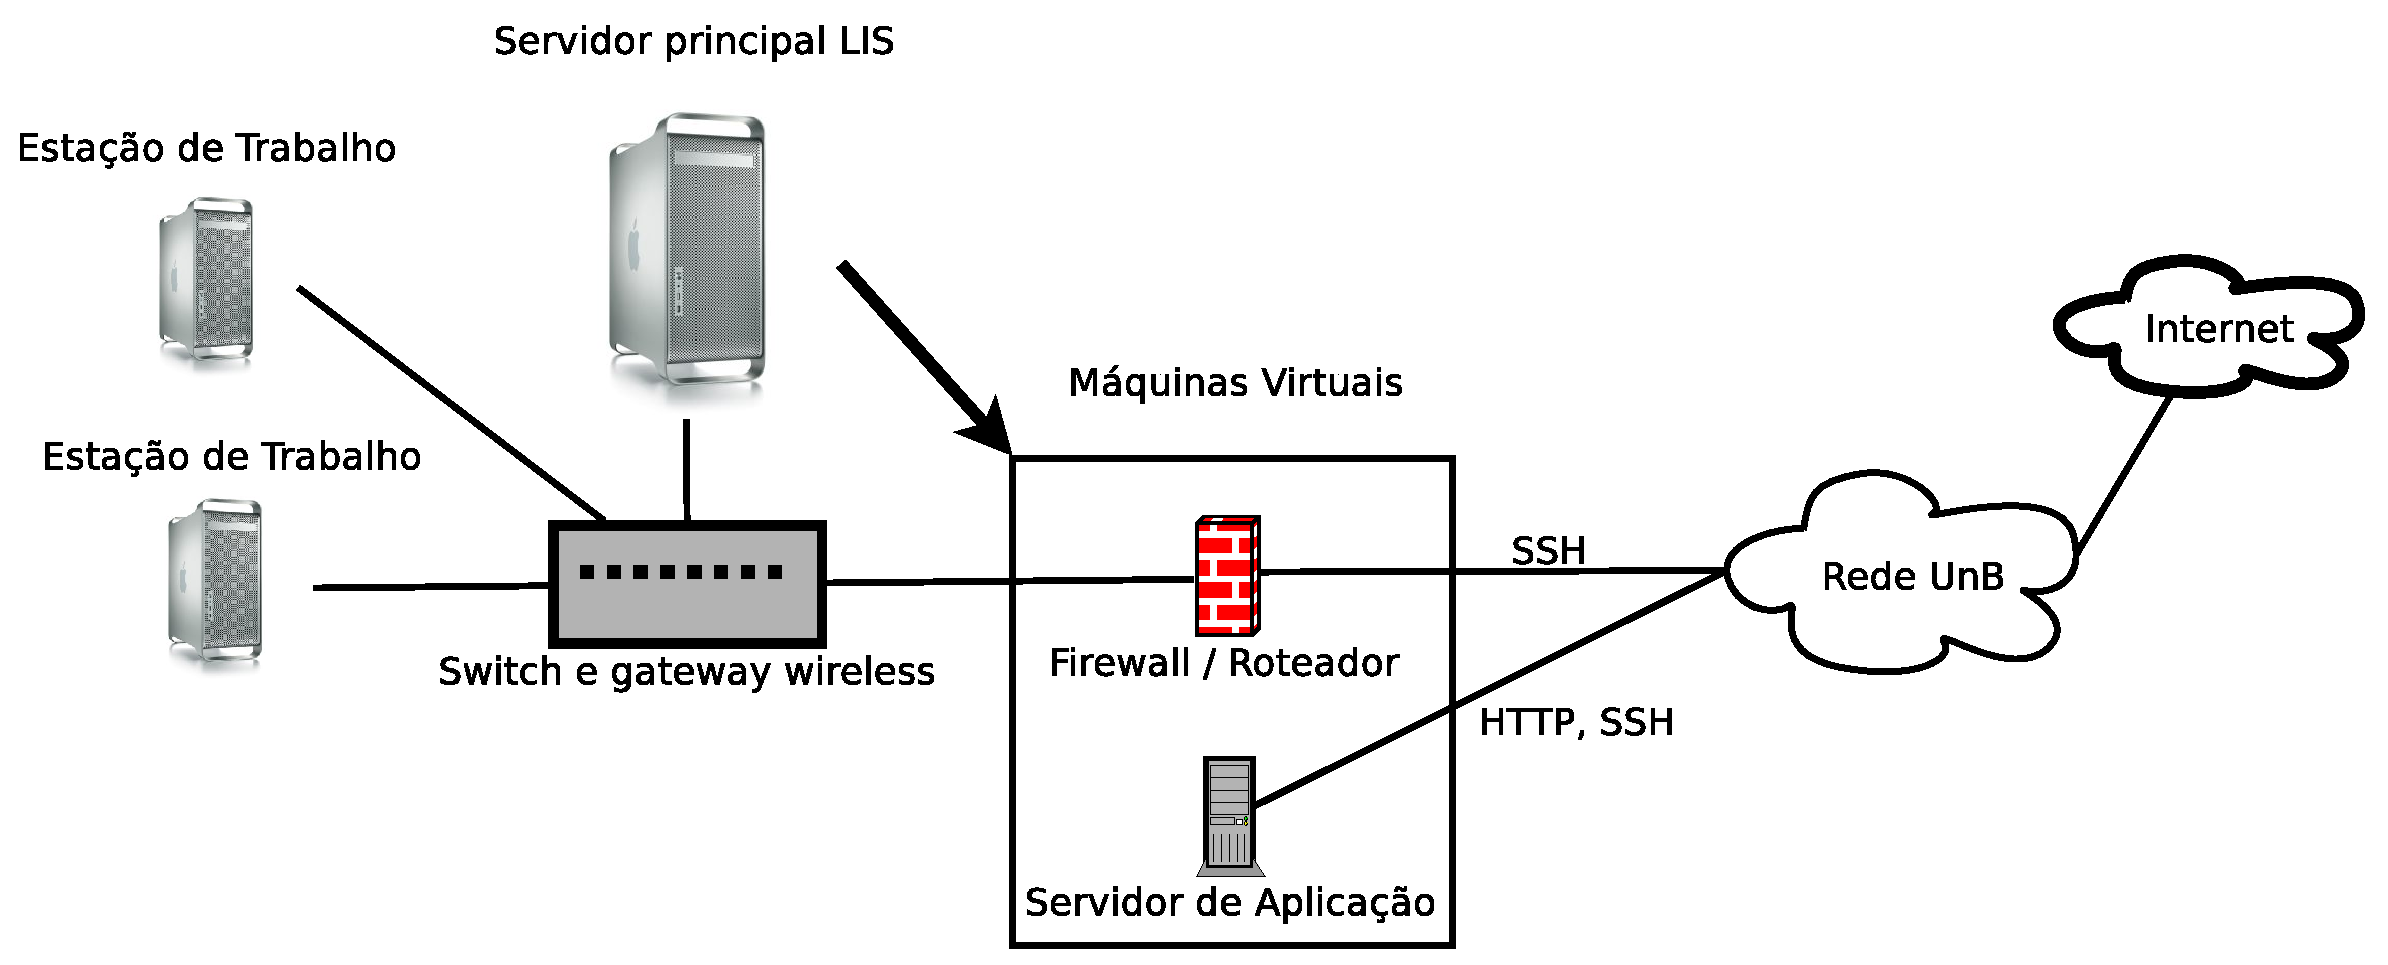
\includegraphics[width=15cm]{figuras/lis_rede.eps}
	\caption{Rede LIS.}
	\label{lis_rede}
\end{figure}

O LPH/FCE foi utilizado para captura de dados de marcha humana. 
Este laboratório está equipado para coletar dados de plataformas de força, eletromiógrafos e de marcadores passivos posicionados no corpo do paciente através de câmeras de vídeo \emph{Oqus-MRI}, usando técnicas de (\emph{Motion Capture - MOCAP}), ver Figura \ref{oqus_mri} na Seção \ref{metodos_analise}. 
Para este trabalho foi utilizado o software \emph{QTM 3.2} da \emph{Qualisys}, ver Figura \ref{visao_qtm} na Seção \ref{metodos_analise}, que é responsável pela coleta de dados \emph{MOCAP}. 

O processo de coleta é demonstrado na Figura \ref{coleta}.

\begin{figure}[ht]
	\centering
	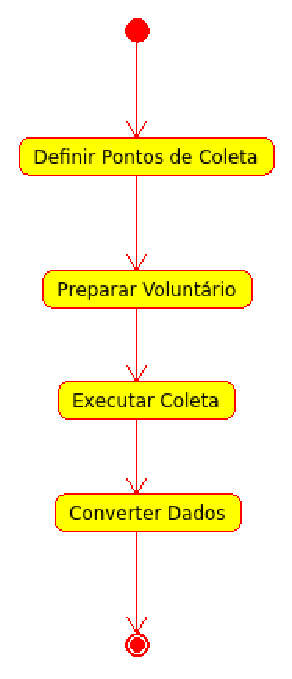
\includegraphics[width=5cm]{figuras/coleta.eps}
	\caption{Processo de coleta de dados.}
	\label{coleta}
\end{figure}

Primeiro deve-se definir o paciente da coleta e determinar o dia para este processo. 
Além disso, também é necessário definir quais os pontos no corpo do paciente devem receber marcadores de superfície. 
O próximo passo se refere a coleta dos dados em si. 
O paciente deve repetir um ciclo de marcha confortável de aproximadamente 5 segundos, por 5 vezes na frente das câmeras.

Quanto aos dados, estes devem ser convertidos para formato adequado à linguagem Octave, que é a mesma opção para converter para o MATLAB. 
Esta opção é própria do QTM. 
O número que o QTM atribui internamente ao marcador é a posição do marcador na matriz gerada durante a exportação. Este número é chamado dentro do QTM de canal. Os dados trazem variáveis espaciais e o erro, com respeito à posição (X, Y, Z) dos marcadores.

A disposição que os dados obtidos neste processo se apresentam, é demonstrada na figura \ref{dados_coleta}.

\begin{figure}[ht]
	\centering
	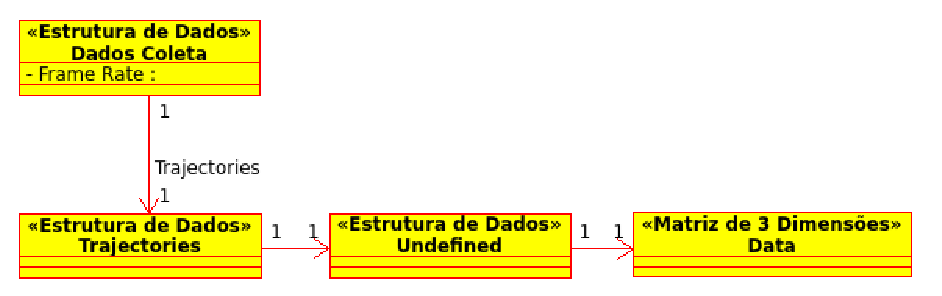
\includegraphics[width=15cm]{figuras/dados_coleta.eps}
	\caption{Dados disponibilizados pelo QTM.}
	\label{dados_coleta}
\end{figure}

São retornados vários dados do QTM, mas os de interesse para o projeto são os que estão na Figura 3. 
O \emph{Frame Rate} é a taxa de coleta dos dados e está em \emph{frames} por segundos. 
A matriz de três dimensões, com dados espaciais dos marcadores passivos de superfície, está disposta da seguinte forma:
\begin{enumerate}
	\item A primeira dimensão tem tamanho variável e representa o número de canais do sistema de coleta, ou seja, cada item representa um marcador;
	\item A segunda dimensão é de tamanho 4 e representa a posição num plano 3D (X, Y, Z) do marcador, mais o erro;
	\item A terceira dimensão é de tamanho variável e representa o número de \emph{frames} coletados numa caminhada específica.
\end{enumerate}

O projeto no qual ocorreu a coleta foi aprovado
pelo Comitê de Ética da Faculdade de Saúde da UnB,
processo N11911/12, ver Anexo \ref{comite_sec}.
